\section{比热的测定}\label{sec:3-5}

比热是物质的特性之一。在许多热学问题上要用到它。所以测定物质的比热是很重要的。

\begin{enhancedline}[1ex]
让我们先举一个实例来说明常用的测定比热的方法。
把质量为 $m_1 = 100$ 克的铜块放在沸水里加热到 $t_{0\,1} = 100$ ℃,
然后把它投进质量为 $m_2 = 88$ 克、温度为 $t_{0\,2} = 15$ ℃ 的水中,
测出它们混合后的共同温度是 $t = 23$ ℃。
水的比热 $c_2$ 是已知的,利用公式 $Q_\text{吸} = c_2m_2(t - t_{0\,2})$,
很容易算出水吸收的热量是 704 卡。
这个热量等于铜块在水中降低温度时放出的热量 $Q_\text{放}$。
公式 $Q_\text{放} = c_1m_1(t_{0\,1} - t)$ 可以变形为
$c_1 = \dfrac{Q_\text{放}}{m_1(t_{0\,1} - t)}$。
把已知数据代入计算,就可以求出铜的比热是 $c_1$ 是 0.091 卡/(克·℃) 。
\end{enhancedline}

上面讲的测比热的方法叫混合法。
用混合法测物质的比热时,应当避免物体放出的热量传递给别的物体。
否则,物体放出的热量就不等于水吸收的热量,给实验带来误差。
为了减少实验误差,人们设计了量热器。

\begin{figure}[htbp]
    \centering
    \begin{minipage}{7cm}
    \centering
    \vspace{1cm}
    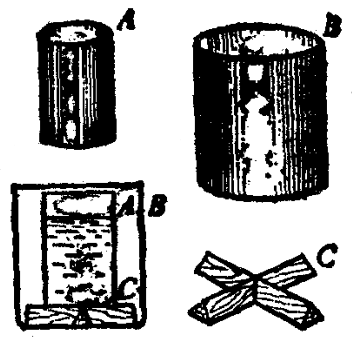
\includegraphics[width=6cm]{../pic/czwl2-ch3-2}
    \caption{量热器的构造}\label{fig:3-2}
    \end{minipage}
    \qquad
    \begin{minipage}{7cm}
    \centering
    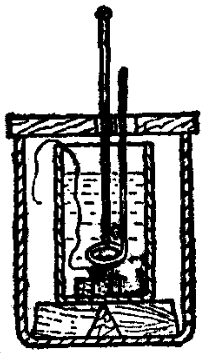
\includegraphics[width=4cm]{../pic/czwl2-ch3-3}
    \caption{用量热器测定物质的比热}\label{fig:3-3}
    \end{minipage}
\end{figure}

通常,量热器是由两个铝筒(或铜筒)$A$、$B$ 和小木架 $C$ 组成的。
木架 $C$ 放在大筒 $B$ 的底上,小筒 $A$ 放在木架 $C$ 上,水就装在小筒 $A$ 里(图 \ref{fig:3-2})。
大筒 $B$ 有个木盖,盖上有两个小孔,一个小孔里插温度计,一个小孔里插搅动器。
实验时,把加热到一定温度、需要测定比热的物体投进小筒的水里,立即把盖盖好(图 \ref{fig:3-3})。
用搅动器搅动水,使水和投进的物体的温度很快变得相同,再从温度计读出它们混合后共同的温度。

量热器的构造使它能够很好地防止热量的散失。
这个道理,同学们可以根据第二章里讲的热传递知识来自己说明。
水和投进的物体混合时,小筒 $A$ 也要吸收热量,在精确的实验中,也要考虑这部分热量。
但是小筒是由比热很小的铝(或铜)制成的,质量又相当小,它吸收的热量比水吸收的少得多。
因此,在初步练习测定比热时,可以不考虑量热器小筒吸收的热量,
而认为水吸收的热量就等于需要测定比热的物体放出的热量。

用混合法不但可以测定比热,还可以测定物体的温度。
例如,我们想知道火炉里的温度而没有合适的温度计,可以找个铁球放到火炉里烧相当长的时间,
使它的温度跟火炉的一样,然后把它取出,立即投入水里,测出混合后的共同温度,
就可以算出混合前铁球的温度,也就知道了火炉里的温度。
如果铁球质量是 100 克,水的质量是 200 克、原来的温度是 15 ℃,
混合后的共同温度是 59 ℃,那么可以算出水吸收的热量,也就等于铁球放出的热量,
是 8800 卡;混合前铁球的温度,也就等于火炉里的温度,是 859 ℃。
详细的计算同学们可以课后自己去做。

